\section{System Overview}
\label{sec: system}

The system architecture is visualized in figure~\ref{fig: architecture}. From the user point of view, our system is divided into two components: developers mode for training gestures and end-user mode for real-time prediction. In a high-level overview, developers using the developer mode supply the system with labeled data with color gloves. The system trains with this labeled data. In the end-user mode, the camera captures raw depth images of the user's naked hands. It then predicts every pixel using the GPU and then pools the predicted pixels to get an estimation of the location of the gesture. Between the two modes, they share a component: feature extraction, which obtains the features for each pixel in the depth image. The implementation of feature extraction in the two modes are different - the training component uses the CPU in an off-line fashion and the end-user prediction component uses the GPU (end-user mode) in an on-demand fashion. 


\begin{figure}
\centering
	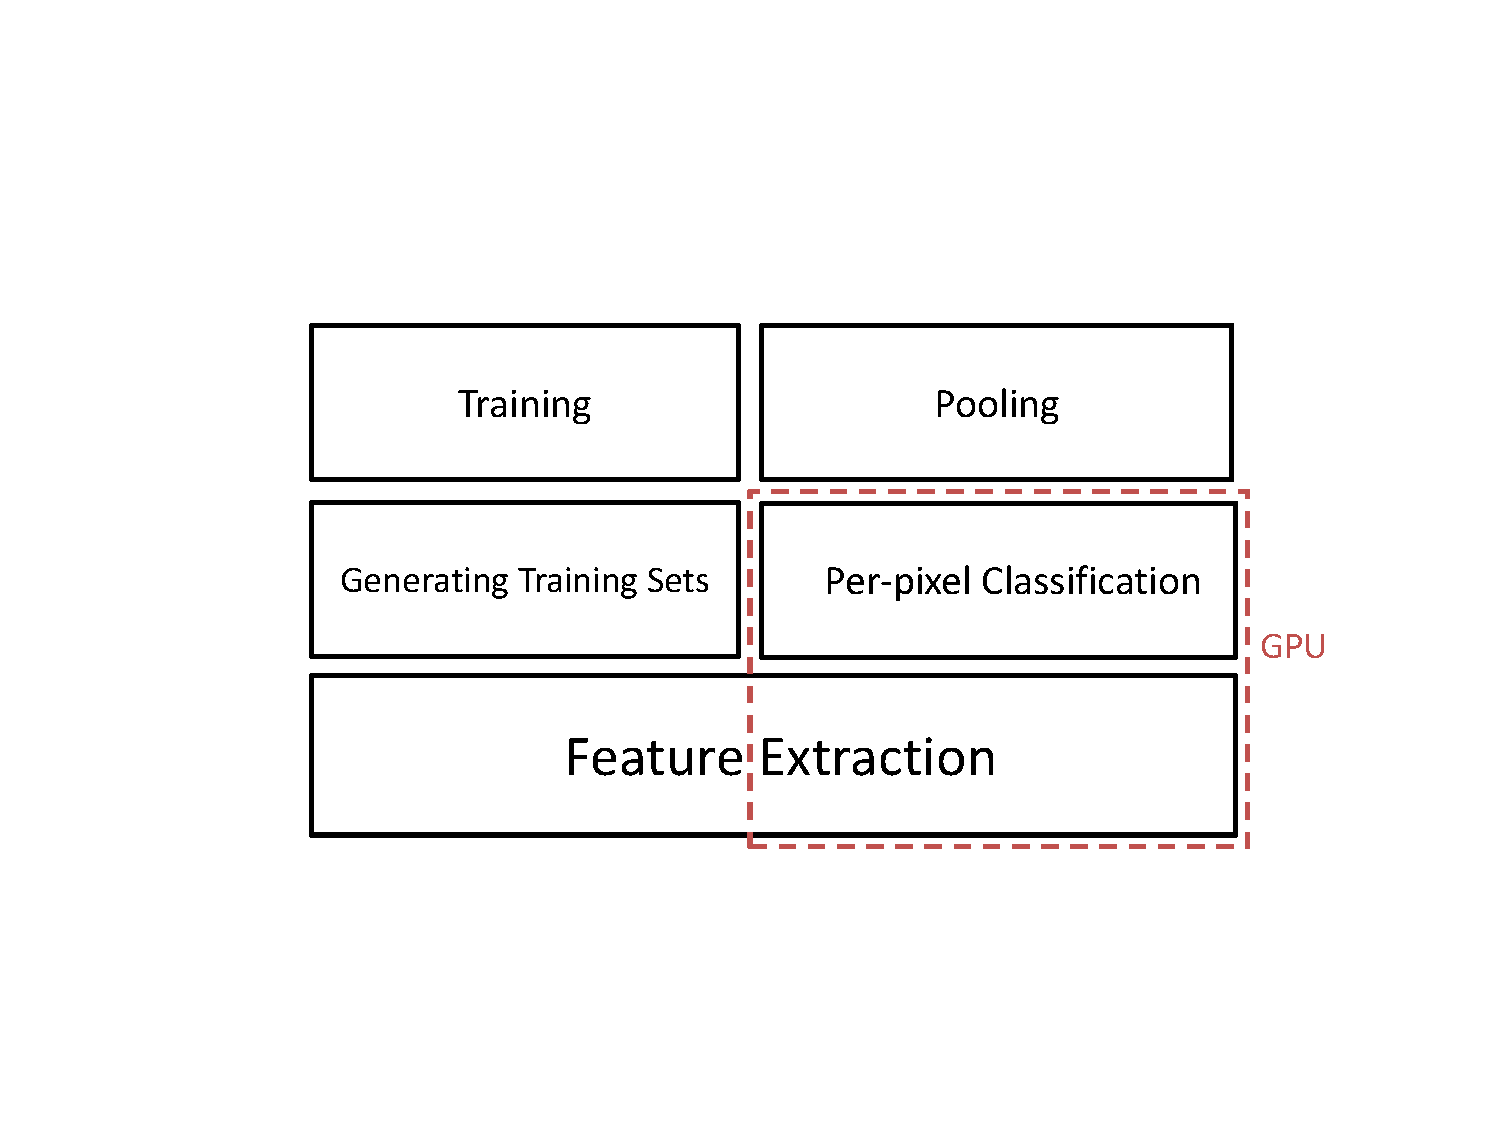
\includegraphics[width=0.5\textwidth]{fig/SystemArchitecture.pdf}
	\caption{An overview of the system architecture}
\label{fig: architecture}
\end{figure}

\subsection{The Kinect Sensor}
The Kinect sensor provides both raw depth image and color image at a maximum frame rate of 30Hz and at 640px $\times$ 480px resolution. Each pixel in the depth image represent the distance from the object to the camera. The error of the depth can be with several millimeters. However, objects can have a shadow where some parts near the object do not have depth value at all. This is an example of realistic noise that may be missing if the training data was generated using computer graphics methods.